\subsection{Unlocking Antenna Magic: The Analyzer Advantage!}

\begin{tcolorbox}[colback=gray!10, colframe=black, title=E4A07] 

Which of the following is an advantage of using an antenna analyzer compared to an SWR bridge?
\begin{enumerate}[label=\Alph*.]
    \item Antenna analyzers automatically tune your antenna for resonance.
    \item \textbf{Antenna analyzers compute SWR and impedance automatically.}
    \item Antenna analyzers display a time-varying representation of the modulation envelope.
    \item All these choices are correct.
\end{enumerate} \end{tcolorbox}

\subsubsection{Related Concepts}

To address this question, we must comprehend the fundamental purposes of an antenna analyzer and an SWR bridge in radio communication systems. 

An antenna analyzer is a specialized tool that can measure important parameters of an antenna system, including Standing Wave Ratio (SWR) and impedance. It allows the operator to adjust the antenna for optimal performance by providing a more comprehensive analysis of the antenna's characteristics over a range of frequencies. This results in an efficient communication system with minimized signal loss.

On the other hand, an SWR bridge is primarily used to measure the SWR, a critical parameter that indicates how well the antenna is matched to the transmission line. While an SWR bridge can provide information about SWR, it often requires manual calculations or observations to infer the impedance.

\subsubsection{Comparison of Antenna Analyzers and SWR Bridges}

\begin{itemize}
    \item \textbf{Functionality:} Antenna analyzers can automatically compute SWR and impedance, thus providing a more holistic view of antenna performance.
    \item \textbf{Ease of Use:} Antenna analyzers often offer a user-friendly interface with real-time graphing capabilities, making it easier to interpret data.
    \item \textbf{Versatility:} Many antenna analyzers can cover a wide frequency range without the need for additional adjustments, unlike SWR bridges, which might be more limited in scope.
\end{itemize}

\subsubsection{Calculation Example}

Assume we have measured the voltage standing waves (VSWR) using our antenna analyzer, and we get a reading of 2:1 VSWR. To compute the impedance we use the following formula:

\[
Z = Z_0 \times \frac{1 + \text{VSWR}}{1 - \text{VSWR}}
\]

where \( Z_0 \) is the characteristic impedance of the transmission line (usually 50 ohms).

Substituting VSWR = 2:

\[
Z = 50 \times \frac{1 + 2}{1 - 2}
\]
\[
Z = 50 \times \frac{3}{-1} = -150 \, \Omega
\]

This calculation indicates a significant mismatch, suggesting the need for antenna adjustment.

\subsubsection{Diagram}

Here is a simple diagram illustrating the relationship between the antenna, transmission line, and the SWR:

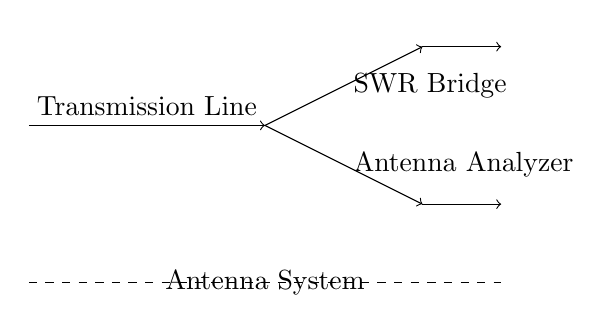
\begin{tikzpicture}
    \draw[->] (0,0) -- (3,0) node[midway, above] {Transmission Line};
    \draw[->] (3,0) -- (5,1) node[midway, right] {SWR Bridge};
    \draw[->] (3,0) -- (5,-1) node[midway, right] {Antenna Analyzer};
    \draw[->] (5,1) -- (6,1) node[midway, above] {};
    \draw[->] (5,-1) -- (6,-1) node[midway, above] {};
    \draw[dashed] (0,-2) -- (6,-2);
    \node at (3,-2) {Antenna System};
\end{tikzpicture}
